%! TEX root = ../main.tex

\chapter{Evaluación}
\label{chap:evaluacion}

En este capitulo se definen las herramientas diseñadas y utilizadas para evaluar
la utilización de los juegos serios en el aprendizaje, estas herramientas están
orientadas a la validación de las hipótesis planteadas en la
sección~\ref{sec:hipotesis}, así como la evaluación de aspectos pedagógicos, de
utilidad y de la participación activa del usuario. Estas herramientas se
utilizan para evaluar a \gls{nombre}.

La evaluación se divide en cinco partes principales:

\begin{itemize}

    \item \textbf{Prueba preliminar de usabilidad:} Es una prueba inicial para
        medir la calidad de la interfaz y la interacción con la misma, esta
        evaluación es realizada con personas no relacionadas al área de
        enfermería, específicamente es realizada a alumnos de la carrera de
        Ingeniería en Informática de la \gls{fpuna}.

        La prueba es llevada a cabo durante el desarrollo de la solución a
        diferencia de las demás, las cuales son realizadas una vez terminada la
        solución.

    \item \textbf{Encuesta de ubicación:} es una encuesta acerca del nivel de
        acceso a la tecnología que poseen los alumnos del 4to año del \Gls{iab},
        de ahora en más la población objetivo, esta encuesta sirve para definir
        la muestra.

        Al finalizar la encuesta de ubicación, se distribuye \gls{nombre} a los
        alumnos que cumplen con los requisitos mínimos y desean participar de
        las pruebas, luego se les realiza la siguientes pruebas para medir su
        nivel de aceptación y aprendizaje, así como el tiempo y frecuencia de
        utilización de la solución.

    \item \textbf{Encuesta para evaluar la solución:} es una encuesta realizada
        a cada sujeto de la muestra, donde se busca la opinión del mismo acerca
        de la solución y factores relacionados a la misma. 

    \item \textbf{Encuesta para evaluar conocimiento:} es un cuestionario que es
        completado por la población de alumnos, donde se mide el conocimiento de
        los mismos, se utiliza a los \revisar{También participan} alumnos que
        no forman parte de la \fixme{muestra}{}, como grupo de control.

    \item Encuesta para evaluar el conocimiento: es un cuestionario cuyo
        objetivo es medir el nivel de conocimiento sobre los temas simulados en
        \gls{nombre}. 
        
        La muestra en esta encuesta es la población entera, los alumnos que no
        utilizaron la aplicación forman un grupo de control.
        
    \item \textbf{Registro de actividades:} Es información almacenada por la
        solución automáticamente, y contiene datos acerca del uso y el desempeño
        del alumno.
        
\end{itemize}

El capitulo define los objetivos de la evaluación, describe brevemente conceptos
transversales a las técnicas utilizadas. Luego, por cada prueba realizada, se
definen las metodologías, métricas y variables utilizadas en cada parte de la
evaluación, y se muestran los resultados de las pruebas, al final del capítulo
se muestran correlaciones entre las variables estudiadas.

%! TEX root = ../main.tex

\section{Métricas generales utilizadas en la evaluación}

En esta sección se describen aquellas métricas que son utilizadas por 
más de una metodología para la evaluación de la solución, las 
cuales se consideran que son importantes detallar.
%En esta sección se definen las métricas que son utilizadas por las pruebas y
%encuestas que forman parte de esta evaluación.

Una de estas métricas es la escala de \textit{Likert}, la cual es una métrica utilizada 
en la \emph{Encuesta para evaluar la solución}
y en la encuesta correspondiente a la \emph{Prueba preliminar de usabilidad}. Otra métrica 
utilizada es la correlación de \textit{Pearson}, esta
métrica es utilizada para medir el grado de relación entre variables de las
encuestas realizadas, los registros de actividades, entre otros.

Cabe destacar que en~\cite{norman2010likert} se demuestra que, aunque el tamaño
de la muestra sea pequeña y los datos no puedan ser distribuidos normalmente o
los datos sean de escalas de tipo \textit{Likert}, los métodos paramétricos como
el análisis de varianza, la regresión y la correlación pueden ser utilizados.


\subsection{Escala de Likert}
\label{sec:likert}

Para la valoración de las variables medidas en la \emph{Prueba preliminar de usabilidad} y 
la {Encuesta para evaluar la solución} se utiliza la escala de
\textit{Likert}\cite{Allen:2007} de 7 valores posibles. La escala de
\textit{Likert} es utilizada para permitir a las personas indicar cuánto están
de acuerdo o en desacuerdo con respecto a ciertos puntos. Los valores
utilizados, son:

\begin{enumerate}
    \item Totalmente en desacuerdo.
    \item En desacuerdo.
    \item Parcialmente en desacuerdo.
    \item Neutral.
    \item Parcialmente de acuerdo.
    \item De acuerdo.
    \item Totalmente de acuerdo.
\end{enumerate}

Una vez valoradas y registradas todas las respuestas y con el objetivo de
eliminar las tendencias en la forma en la que son completadas las
encuestas\cite{Fischer2010} se utiliza el método de \emph{Doble Estandarización}
recomendado en~\cite{Pagolu2011}. Este método, consiste en dos
estandarizaciones, la primera por fila, que en este caso representa a los
individuos y la segunda por columna donde cada columna representa una de las
diferentes preguntas de la encuesta.

Siendo:
\begin{itemize}
	\item $\min_i$ la respuesta de menor valor del usuario $i$.
	\item $\max_i$ la respuesta de mayor valor del usuario $i$.
\end{itemize}

Para cada respuesta $s$ del usuario $i$, el valor ajustado, por la primera 
normalización, $s_1$ se define como:

\begin{equation}
s_1{_i}=\frac{s-\min_i}{\max_i-\min_i}
\end{equation}

%\observacion{Considerar resumir}
Y luego siendo:
\begin{itemize}
	\item $groupmin_i$ la respuesta ajustada de menor valor en el grupo $i$.
	\item $groupmax_i$ la respuesta ajustada de mayor valor en el grupo $i$
\end{itemize}

Para cada respuesta ajustada $s_1{_i}$ del usuario $i$, el valor ajustado $sa_i$ se
define como:	

\begin{equation}
sa_i=\frac{s_{1_i}-groupmin_i}{groupmax_i-groupmin_i}
\end{equation}

Obteniendo así un valor normalizado, tanto por individuo, como por pregunta, en
el rango $0$ y $1$.

Para la valoración absoluta de cada  item se utiliza la media de cada columna o
respuesta a una pregunta de la encuesta.

Siendo:
\begin{itemize} 
\item $r_{k_i}$ la respuesta del usuario $i$ a la pregunta $k$.
\item $t_k$ la cantidad total de usuarios que respondieron la pregunta $k$.
\end{itemize}

El puntaje promedio de cada pregunta o item evaluado  $p_k$ en la encuesta se
define como:

\begin{equation}
p_k = \frac{\sum_{i=1}^n{r_{k_i}}}{t_k}
\end{equation}

%\subsubsection{Manejo de información faltante}
%\label{sec:informacion_faltante}
%\observacion{No repetir tanto existe}
%
%En toda encuesta pueden haber preguntas que no son respondidas por los encuestados, 
%en este tipo de situaciones existen tres posibles formas de categorizar el 
%patrón de ocurrencia de la falta de 
%respuestas\cite{leite2010performance,tsikriktsis2005review}:
%
%\begin{description}
%    \item[Información faltante completamente aleatoria:] cuando la información
%        faltante es independiente de la variable medida y de otras variables.
%    \item[Información faltante aleatoria:] cuando la información faltante depende
%        de otras variables, pero no de la variable en sí. 
%    \item[Información faltante no aleatoria:] cuando hay una relación entre la
%        información faltante y el valor de la variable.
%\end{description}
%
%Una vez categorizado el patrón de ocurrencia, existen a su vez tres
%mecanismos~\cite{tsikriktsis2005review} principales para lidiar con información
%faltante como son la eliminación, el reemplazo y los  procedimientos basados en
%modelo.~\cite{tsikriktsis2005review} recomienda utilizar un mecanismo de
%reemplazo para escalas del tipo \textit{Likert}.
%
%Las técnicas de reemplazo se clasifican en tres grandes
%grupos\cite{tsikriktsis2005review}:
%\begin{enumerate*}[label=\itshape\alph*\upshape)]
%\item basadas en el promedio,
%\item basadas en regresión, e,
%\item imputación \emph{hot deck}.
%\end{enumerate*}
%
%\fixme{De estas técnicas se seleccionó la sustitución}{Resaltar}. Basada por
%promedio ya que las relaciones entre las variables son bajas y los datos
%faltantes son menos del $10\%$. La sustitución basada por promedio se divide
%nuevamente en tres grupos\cite{tsikriktsis2005review}; promedio
%\begin{enumerate*}[label=\itshape\alph*\upshape.]
%\item total,
%\item del subgrupo, y,
%\item por caso.
%\end{enumerate*}
%
%La sustitución por promedio total es elegida debido a que la relación entre la
%variable que falta y las demás variables en los datos es relativamente baja, es
%fácil de usar y retiene la muestra. La sustitución por promedio total se realiza
%obteniendo el promedio de todas las respuestas de la pregunta cuya respuesta
%falte, la sustitución de subgrupo es similar, solo que se limita a aquellos
%sujetos del mismo subgrupo del sujeto que no respondió, y finalmente, la
%sustitución por caso, es el promedio de las respuestas válidas del sujeto.

\subsection{Correlación de variables aleatorias}
\label{sec:correlacion}

Las correlaciones se utilizan durante una etapa exploratoria o de observación de
la investigación para determinar las variables que tienen al menos una relación
estadística con cada uno de los diseños experimentales. Las correlaciones
también se utilizan para determinar el grado de asociación entre variables
dependientes e independientes. Por otro lado, el coeficiente de correlación se
utiliza comúnmente para cuantificar el grado de asociación entre dos variables
\cite{BoslaughStatistics2008}.

La correlación de Pearson\cite{BoslaughStatistics2008} mide la relación que
existe entre dos variables, $X$ e $Y$, el mismo esta comprendido entre $-1$ y
$1$, en su punto más bajo ($-1$) indica que una de las dos variables crece mientras
la otra decrece, y en su punto más alto ($1$), indica que ambas crecen o
decrecen conjuntamente, el valor $0$, indica que no existe una relación entre
ambas variables.

El coeficiente para las variables $X$ e $Y$ está dado por:

\begin{equation}
r = \frac{\sum_{i=1}^n{(\frac{x_i-\bar{x}}{s_x})({\frac{y_i-\bar{y}}{s_y}})}}%
{n - 1}
\end{equation}

donde:

\begin{itemize}
    \item ($x_i$, $y_i$) es el conjunto de coordenadas de las variables $X$ e $Y$.
    \item $\bar{x}$ es la media de la variable $X$.
    \item $\bar{y}$ es la media de la variable $Y$.
    \item $s_x$ es la desviación estándar de la variable $X$.
    \item $s_y$ es la desviación estándar de la variable $Y$.
    \item $n - 1$ son los grados de libertad.
\end{itemize}

\section{Objetivos}


\begin{itemize}
    \item Determinar el nivel de aceptación de la propuesta.
    \item 

\end{itemize}

\section{Prueba preliminar de usabilidad}
\label{sec:interfaz}

Durante el desarrollo de la solución se realizó una prueba para evaluar la 
interfaz de usuario, específicamente buscando la retroalimentación de usuarios 
acostumbrados a tecnología similar a la utilizada en la solución.

Esta prueba ayuda en el proceso de diseño e implementación de la solución con 
las características mencionadas en los objetivos del trabajo y acorde a los 
requerimientos. De esta manera se pueden identificar los aspectos que deben 
ser mejorados.

La prueba consta de dos partes importantes involucradas en la recolección
de datos para su posterior análisis. Estas partes son las siguientes:

\begin{description}

\item[Simulación:] luego de una explicación acerca de las funciones y manejos
    generales de la solución por parte de los encargados de la prueba, cada usuario
    completa una tarea que consiste en realizar el procedimiento de venopunción con la 
    solución, como ayuda, recibe una hoja con una lista de todos los pasos 
    necesarios para llevar a cabo el procedimiento.
    	
    Las simulaciones son grabadas con programas de captura de pantalla, así
    como por detectores de eventos táctiles.
    	
\item[Encuesta:] posteriormente se le provee una encuesta a cada
    usuario la cual es utilizada para obtener una idea general acerca de la
    calidad de la simulación según la percepción de los usuarios. Esta encuesta 
    contiene preguntas que son medidas mediante la escala de tipo Likert. 

\end{description} 

\subsection{Muestra}

La prueba de usabilidad de la interfaz de usuario se realiza con alumnos de la
carrera de Ingeniería en Informática de la \Gls{fpuna}, sin experiencia previa
tanto con la solución como con los procedimientos simulados, pero sí
familiarizados con la utilización de dispositivos móviles. La muestra no
requiere de sujetos que sean parte del \emph{población objetivo} ya que sólo
está orientada a mejorar aspectos de interfaz de usuario y no el contenido de la
solución, además se considera que la muestra puede brindar una evaluación más
crítica debido a su familiarización con interfaces similares a la de la
solución.

El número de muestras tomadas fue 8, ya que según~\cite{nielsen2000} son
necesarios al menos $5$ participantes para poder obtener resultados
significativos en una prueba de usabilidad. Además,~\cite{ritch2009} asegura que
la teoría de~\cite{nielsen2000} es verdadera especialmente para pruebas simples. 

Se fundamenta el número de participantes, y que es una prueba sencilla, ya que:

\begin{itemize}

\item La prueba no debería tomar más de $10$ minutos en ser realizada.

\item Se busca solamente obtener información acerca de la interfaz, y no el
    funcionamiento en sí de la simulación, pues los usuarios no son expertos en
    el área y no tienen conocimiento acerca las tareas.

\item No se busca evaluar el aspecto pedagógico de la solución sino sólo su interfaz gráfica.
%\item No se busca medir el aprendizaje del usuario en temas no relacionados a la
%    interfaz, es decir, no se mide el aprendizaje del usuario en el tema
%    simulado\revisar{No se entiende, no se mide el aspecto pedagógico solo la
%    interfaz gráfica de la simulación}.

\item El procedimiento de enfermería a realizarse con la solución está bien definido 
y los pasos necesarios están a disposición del usuario en todo momento.

\end{itemize}

\subsection{Variables}
\label{sec:evaluacion_interfaz_variables}

Antes de definir las variables, se deben primero definir los conceptos 
relacionados a los tipos de acciones que pueden realizarse sobre el paciente 
virtual en la solución, los mismos son:

%\observacion{Cual se encarga del diseño de la simulación?}
\begin{itemize}
\item \textbf{Acción por menú contextual:} se refiere a las acciones que el usuario 
    puede realizar utilizando el menú contextual que aparece sobre cada uno de los elementos 
    disponibles en la solución.
\item \textbf{Acción por menú de la \Gls{gui}:} se refiere a las 
    acciones que el usuario puede realizar seleccionando una opción en los menús 
    principales que presenta la interfaz de la solución.
\item \textbf{Acción con elemento:} se refiere a las actividades que el usuario 
    puede realizar cuando tiene seleccionado un elemento y que no involucre el 
    uso del menú contextual.
\end{itemize}


Las variables medidas durante la realización de la tarea con la solución son las
siguientes:

%\observacion{No repetir tanto la descripción en el título}

\begin{itemize}

\item \textbf{Tiempo de realización de la primera acción por tipo:} cuanto tiempo 
	le toma al usuario realizar la primera vez una acción agrupado por tipo (por menú 
	contextual, por menú de la \Gls{gui}, con elementos).

%\item \textbf{Tiempo de realización de la primera acción por menú contextual:} 
%    cuanto tiempo le toma al usuario realizar una acción por menú contextual la 
%    primera vez.
%
%\item \textbf{Tiempo de realización de la primera acción por \Gls{gui}:} cuanto 
%    tiempo le toma al usuario realizar una acción por menú de 
%    interfaz gráfica de usuario la primera vez.
%    
%\item \textbf{Tiempo de realización de la primera acción por herramienta:} cuanto 
%    tiempo le toma al usuario realizar una acción por herramienta la primera vez.

\item \textbf{Tiempo de realización de las siguientes acciones por tipo:} cuanto tiempo 
	le toma al usuario realizar las siguientes veces una acción agrupado por 
	tipo (por menú contextual, por menú de la \Gls{gui}, con elementos).
 
%\item \textbf{Tiempo de realización de las siguientes acciones por menú contextual:} 
%    cuanto tiempo le toma al usuario realizar una acción por menú 
%    contextual las siguientes veces.
%
%\item \textbf{Tiempo de realización de las siguientes acciones por \Gls{gui}:} 
%    cuanto tiempo le toma al usuario realizar una acción 
%    por interfaz gráfica de usuario las siguientes veces.
%
%\item \textbf{Tiempo de realización de las siguientes acciones por herramienta:} 
%    cuanto tiempo le toma al usuario realizar una acción por herramienta 
%    las siguientes veces.

\item \textbf{Tiempo total:} se refiere al tiempo empleado por el usuario para 
    completar la tarea asignada.

\item \textbf{Número de pasos realizados:} cantidad de pasos requeridos en la tarea 
    que son realizados por el usuario en la simulación. 

\item \textbf{Cantidad de movimientos espaciales por tipo:} número de veces en que se 
    modifica el estado de la cámara para realizar las acciones deseadas agrupados por 
    tipo (desplazamiento, acercamiento/alejamiento).

%    \observacion{Esto donde entra?}

\end{itemize}

En cuanto a la encuesta, las siguientes son las variables que fueron consideradas 
y medidas:

\begin{itemize}

\item \textbf{Calidad gráfica:} realismo y calidad de los modelos utilizados.

\item \textbf{Interacción:} desenvolvimiento en el entorno y utilización del 
    hardware.

\item \textbf{Interacción con objetos:} utilización errónea de objetos.

\item \textbf{Características del entorno:} realismo del escenario y de los 
    objetos utilizados.

\item \textbf{Usabilidad de la interfaz:} facilidad de uso de las opciones 
    proveídas por la interfaz.

\item \textbf{Integración con el hardware:} facilidad de uso de la solución con 
    un dispositivo móvil. 

\end{itemize}

\subsection{Métricas}

Para la medición de las variables relacionadas a la encuesta,  se utiliza la escala
de Likert con la \emph{Doble estandarización} explicada en la
sección~\ref{sec:likert}. 

En cambio, para la medición de las variables relacionadas a la interacción del usuario con 
la solución se utilizan las grabaciones registradas durante las pruebas y las
las siguientes métricas:

%Para el análisis de la encuesta realizada a los usuarios, se utiliza la escala
%de Likert con la \emph{Doble estandarización} explicada en la
%sección~\ref{sec:likert}, y en el análisis de la interacción del usuario con la
%solución se utilizan las grabaciones registradas durante la prueba.
%
%Haciendo uso de las variables descriptas anteriormente, las métricas
%utilizadas son las siguientes:

\begin{itemize}
    
\item \textbf{Tiempo promedio de realización de las siguientes acciones por menú contextual:} 
    se obtiene dividiendo la cantidad total de tiempo empleado en realizar acciones por menú 
    contextual por el número de veces que se realizaron esas acciones, sin considerar la primera 
    vez. 
    
\item \textbf{Tiempo promedio de realización de las siguientes acciones por \Gls{gui}:} 
    se obtiene dividiendo la cantidad total de tiempo empleado en realizar acciones por \Gls{gui} 
    por el número de veces que se realizaron esas acciones, sin considerar la primera 
    vez. 
    
\item \textbf{Tiempo promedio de realización de las siguientes acciones por herramienta:} 
    se obtiene dividiendo la cantidad total de tiempo empleado en realizar acciones por 
    herramienta por el número de veces que se realizaron esas acciones, sin considerar la 
    primera vez. 
    
\item \textbf{Promedio de pasos correctos:} se obtiene dividiendo la cantidad de 
    pasos requeridos realizados por los usuarios sobre la cantidad de pasos requeridos. 
    
\item \textbf{Promedio de movimientos por tipo:} se obtiene dividiendo el número de 
    movimientos que fueron realizados agrupados por tipo (desplazamiento, acercamiento/
    desplazamiento) por la cantidad de usuarios.
    
\item \textbf{Promedio del tiempo total:} se obtiene dividiendo el tiempo total empleado 
    por los usuarios para completar la tarea asignada por el número de usuarios.

\end{itemize}

\subsection{Resultados obtenidos}
\label{sec:res_interfaz}

A continuación de muestran y analizan los resultados obtenidos en la prueba. Los resultados 
se dividen en \emph{simulación} y \emph{encuesta} para una mejor comprensión.

\subsubsection{Simulación}

Las grabaciones realizadas a las sesiones de los usuarios se utilizan para medir
el grado de facilidad de aprendizaje de la interfaz de usuario.

Dados los tres tipos de acciones descritos en~\ref{sec:evaluacion_interfaz_variables}, la
tabla~\ref{tab:interfaz_tiempo_acciones} muestra el tiempo, en segundos,
que le tomo a cada usuario realizar una acción la primera vez y 
el tiempo que les tomo en promedio las demás veces, para cada uno de los tipos 
de acciones.

%\observacion{Hacer énfasis en la comparación entre el primer y los siguientes}

\begin{table}[!hbt]
\centering
\begin{tabular}{|c|c|c|c|c|c|c|}
\hline
& \multicolumn{2}{c|}{\textbf{Menú Contextual}} &
\multicolumn{2}{c|}{\textbf{Menú de la Interfaz}} & \multicolumn{2}{c|}{\textbf{Herramienta}}\\
\hline
\textbf{Usuario}  & \textbf{Primera} & \textbf{Siguientes} & \textbf{Primera} & \textbf{Siguientes} & \textbf{Primera} & \textbf{Siguientes} \\
\hline 1          & 8                & 2.25                & 3                & 9.14                & 11               & 3.0 \\
\hline 2          & 30               & 7.00                & 4                & 3.57                & 7                & 4.5 \\
\hline 3          & 5                & 2.25                & 5                & 1.86                & 1                & 1.0 \\
\hline 4          & 2                & 13.00               & 4                & 2.00                & 1                & 0.5 \\
\hline 5          & 18               & 2.75                & 6                & 4.43                & 6                & 3.0 \\
\hline 6          & 4                & 14.25               & 11               & 7.86                & 13               & 4.0 \\
\hline 7          & 5                & 8.00                & 4                & 4.71                & 20               & 2.5 \\
\hline 8          & 3                & 2.33                & 10               & 3.57                & 3                & 6.5 \\
\hline
\textbf{Promedio} & \textbf{9.38}    & \textbf{6.37}       & \textbf{5.88}    & \textbf{4.64}       & \textbf{7.75}    & \textbf{3.125} \\
\hline
\end{tabular}
\caption{Tiempo por acciones la primera vez y las siguientes veces que se realizo}
\label{tab:interfaz_tiempo_acciones}
\end{table}

En la tabla~\ref{tab:interfaz_tiempo_acciones} se observa consistentemente una 
mejora en el tiempo de realización de un tipo de acción con respecto a la primera vez 
que es realizada. 

\begin{filecontents}{interfazuso.dat}
n   p       s
1	9.38	6.48
2   5.88	4.64
3   7.75	3.13
\end{filecontents}
\pgfplotstableread{interfazuso.dat}{\InterfazUso}

\begin{figure}[H]
    
        \centering
        \begin{tikzpicture}[scale=.8]
           \begin{axis}[ybar,%
              legend pos=outer north east,
              xmin=1,
              xmax=3,
              x=2.5cm,
              enlarge x limits={abs=1cm},
              xtick=data,
              symbolic x coords={0,1,2,3,4},
              ymin=0,ymax=10,
              %ytick={0,2,4,6,8,10},
              xticklabels={Contextual,Interfaz,Herramienta},
              ylabel= Tiempo (s),
              xlabel= Tipo de acción,
              bar width=10pt,
              %enlarge x limits={abs=2},
                ]   
        \addplot[color=blue!90,ybar,fill=blue!55,area legend] table [x = {n}, y = {p}] {\InterfazUso};
        \addlegendentry{Primer}
        \addplot[color=red!90,ybar,fill=red!55,area legend] table [x = {n}, y = {s}]
        {\InterfazUso};
        \addlegendentry[align=left]{Promedio \\ siguientes}
        \end{axis}
        \end{tikzpicture}
        \caption{Tiempo por tipo de acción}
        \label{fig:interfaz_tiempo_acciones}
\end{figure}

En la figura~\ref{fig:interfaz_tiempo_acciones} se observa como en promedio el
usuario aprende, y en las siguientes acciones similares demora menos tiempo,
este es un factor importante y es el objetivo de esta prueba pues muestra que la
interfaz es fácil de usar, y con tres tipos de acciones, el usuario puede
utilizarla sin mayores inconvenientes. Se observa una mejoría del $30\%$ en las
\emph{Acciones por menú contextual}, $21\%$ en las \emph{Acciones por menú de la
    \Gls{gui}} y finalmente, una mejoría del $60\%$ en las \emph{Acciones con elementos}.


\begin{table}[hbt]
\centering
\small
\begin{tabular}{lrrr}
\toprule
\textbf{Jugador}  & \textbf{Desplazamiento} & \textbf{Acercamiento/alejamiento} & \textbf{Total} \\
\midrule
1        & 18         & 2    & 20 \\
2        & 7          & 8    & 15 \\
3        & 14         & 12   & 26 \\
4        & 9          & 14   & 23 \\
5        & 5          & 8    & 13 \\
6        & 14         & 4    & 18 \\
7        & 16         & 3    & 19 \\
8        & 4          & 3    &  7 \\
\midrule
\textbf{Promedio} & \textbf{10,88}      & \textbf{6,75} & \textbf{17,63} \\
\bottomrule
\end{tabular}
\caption{Cantidad de movimientos espaciales}
\label{tab:interfaz_cantidad_espaciales}
\end{table}

En la tabla~\ref{tab:interfaz_cantidad_espaciales} se observa la cantidad de
movimientos espaciales realizados por los usuarios, se observa que en promedio
se desplazaron $10,88$ veces por el escenario, y $6,75$ veces acercaron o
alejaron la cámara del paciente.

No existe una cantidad mínima o máxima de movimientos que el usuario debe realizar para acercar, 
alejar o desplazar la cámara. Los datos mostrados en la tabla~\ref{tab:interfaz_cantidad_espaciales} 
muestran que no son necesarias demasiados movimientos. Teniendo en cuenta esta información y la 
proveída en la tabla~\ref{tab:interfaz_tiempo_total}, se concluye 
que en promedio los usuarios realizan $1,7$ movimientos por minuto.

\begin{table}[!hbt]
\centering
\small
\begin{tabular}{lrrr}
\toprule
\textbf{Alumno} & \textbf{Tiempo (min)} \\
\midrule
1        & 8:32 \\
2        & 6:03 \\
3        & 8:33 \\
4        & 5:17 \\
5        & 6:55 \\
6        & 8:40 \\
7        & 7:03 \\
8        & 10:27 \\
\midrule
\textbf{Promedio} & \textbf{7:41} \\
\bottomrule
\end{tabular}
\caption{Tiempo de prueba por usuario}
\label{tab:interfaz_tiempo_total}
\end{table}

El tiempo total que se observa en la tabla~\ref{tab:interfaz_tiempo_total},
muestra que en promedio a cada alumno le tomo $7:41$ minutos realizar todos los
pasos especificados, es importante notar que este tiempo incluye el tiempo de
adaptación. 

La tabla~\ref{tab:interfaz_acciones} nos muestra la cantidad de pasos
realizados por los alumnos de un total de 19. Se observa que en promedio 
realizaron $16.75$ pasos.

\begin{table}[htb]
\centering
\small
\begin{tabular}{lrrr}
\toprule
\textbf{Alumno} & \textbf{Pasos realizados (19)} \\
\midrule
1 & 19 \\
2 & 15 \\
3 & 18 \\
4 & 15 \\
5 & 18 \\
6 & 16 \\
7 & 19 \\
8 & 14 \\
\midrule
\textbf{Promedio} & \textbf{16,75} \\
\bottomrule
\end{tabular}
\caption{Pasos realizados por alumno}
\label{tab:interfaz_acciones}
\end{table}



\subsubsection{Encuesta}


La encuesta es utilizada para obtener el grado de disconformidad de los usuarios
con respecto a la solución. Se utiliza la disconformidad para resaltar los
puntos débiles, así, aquellas variables que tengan el mayor porcentaje serán las
que deban ser mejoradas.


En la tabla~\ref{tab:interfaz_disconformidad_metrica} se observan que las
mayores disconformidades son la usabilidad de la interfaz de usuario que llega
al $51\%$, la interacción de los usuarios con el entorno que llega al $50\%$ y
la interacción con los objetos que llega al $49\%$. Otras disconformidades con
menor porcentaje son las características del entorno con un  $33\%$, la
integración con el hardware con un $27\%$ y por último la calidad gráfica con un
$17\%$.


\begin{table}[htb]
\centering
\begin{tabular}{lr}
\toprule
\textbf{Variable} & \textbf{Disconformidad (0-1)}\\
\midrule
Calidad Gráfica         & 0.17 \\
Interacción Entorno     & 0.50\\
Interacción Objetos     & 0.49\\
Características Entorno & 0.33\\
Usabililidad Interfaz   & 0.51\\
Integración Hardware    & 0.27\\
\bottomrule
\end{tabular}
\caption{Disconformidad por variable}
\label{tab:interfaz_disconformidad_metrica}
\end{table}

%La conclusión de esta prueba de interfaz, es que si bien, pudo ser utilizada sin
%mayores inconvenientes, existe un alto grado de disconformidad con la interfaz,
%además cabe resaltar, los sujetos de prueba son personas acostumbradas al uso de
%tecnologías similares. Otros puntos débiles encontrados en esta prueba son la
%interacción con el entorno y  con los objetos.

Como consecuencia de los resultados obtenidos, la usabilidad de interfaz y la interacción con objetos y 
con el entorno son mejoradas para obtener la versión final de la solución que es utilizada por 
los estudiantes de enfermería. Las demás pruebas mencionadas en este capítulo son realizadas con 
la versión final de la solución.
%elementos sufren modificaciones a fin de su utilización con usuarios no
%técnicos.

%Las demás pruebas mencionadas en este capítulo son realizadas con la versión
%final de la solución, la cual es obtenida luego de las mejoras realizadas a los
%puntos débiles detectados por esta prueba.

%! TEX root = ../main.tex

\section{Encuesta de ubicación}
\label{sec:ubicacion}

Para recabar información acerca del nivel de acceso  de los alumnos a la
tecnología, se realiza una encuesta que cuenta con diez preguntas, las cuales
buscan conocer sobre el modelo de dispositivo móvil, el acceso a
Internet, y la predisposición de cada alumno a ayudar en la prueba.

Con los resultados de la encuesta de ubicación tecnológica, se seleccionan
aquellos alumnos que posean dispositivos móviles que superan o igualan las
especificaciones descriptas más adelante. De esta encuesta se obtendrán los 
usuarios que formarán parte de la población que evaluará la versión final de 
la solución.

\subsection{Muestra}

En el año $2014$, el \Gls{iab} cuenta con $124$ alumnos en el cuarto año distribuidos en
tres secciones, el cual es considerado el \emph{Universo}. De los 124, 93 de
ellos estuvieron interesados en participar de la prueba y completaron la encuesta.

\subsection{Variables}

Se definen $2$ factores necesarios para que un alumno pueda ser considerado como
sujeto de prueba, el primero es la predisposición del mismo a participar de la
prueba y el segundo es que posea un dispositivo móvil que supere los requisitos
mínimos. Además de estos dos factores, la conexión a internet es requerida, pues 
los registros de actividad de cada dispositivo deben ser enviados y almacenados 
para su posterior interpretación y análisis. A continuación se describen las variables 
consideradas.


\begin{itemize}

\item \textbf{Requisitos mínimos:} son aquellos requerimientos técnicos con los que 
    debe cumplir completamente el dispositivo móvil del usuario para que la 
    solución tenga un desempeño que garantice una experiencia fluida a la hora de 
    utilizarla. Estos requisitos son:
    \begin{itemize}
        %%\item Sistema Operativo Android $4.0$ o superior
        \item Memoria ram de $512$MB o superior.
        \item Velocidad de procesador de $800$ GHz o superior.
        \item \Gls{gpu} Mali 400 o superior.
        %\item Conexión frecuente a internet.
    \end{itemize}
    Los requisitos de \textit{hardware} mencionados, son requeridos por las
    características de la simulación, una \Gls{gpu} es requerida por los gráficos en 
    tres dimensiones.

\item \textbf{Tipo de acceso a internet:} el tipo de acceso a internet que posee el 
    usuario en su dispositivo móvil. Puede ser una de las siguientes opciones:
    plan post-pago, paquetes pre-pago, acceso ocasional y sin acceso.
    
\item \textbf{Sistema Operativo:} se refiere al tipo de sistema operativo que posee 
    el dispositivo móvil del usuario.

    \observacion{Donde se menciona?}
    
\end{itemize}

\subsection{Métricas}

Las métricas utilizadas para estudiar los datos recogidos son sencillas ya que
sólo buscan determinar la población que evaluará la solución, estas métricas son
las siguientes:

\begin{itemize}
\item Porcentaje de encuestados con dispositivos móviles que cumplen y que no cumplen con 
los requisitos mínimos.
\item Porcentaje del tipo de acceso a internet de los usuarios.
\item Porcentaje del tipo de sistema operativo que poseen los dispositivos móviles de los 
encuestados.
\end{itemize}



%! TEX root = ../main.tex

\section{Encuesta para evaluar la solución}
\label{sec:subjetiva}

Al final del período de prueba de la solución cada alumno que forma parte de la muestra
completa una encuesta con $31$ preguntas que se utilizan para validar las
consideraciones de diseño, las cuales fueron explicadas en el capítulo~\ref{chap:requerimientos}
y para medir sus apreciaciones sobre otros aspectos de la solución que serán
detallados más adelante en esta sección. 

Las preguntas están agrupadas en dos, el primer grupo cuenta con $27$ preguntas
cerradas, es decir de una sola respuesta en una lista de opciones, el segundo
grupo cuenta con $4$ preguntas abiertas, es decir los encuestados pueden dar
respuestas libres a las preguntas. 

De esta forma, se busca identificar las fortalezas y debilidades de la solución,
además de evaluar la solución en cuanto a factores de exploración,
representación, motivación, inmersión, retroalimentación y pedagogía, de acuerdo
a las apreciaciones de los miembros de la muestra.

\subsection{Muestra}

La encuesta es entregada a los $11$ alumnos de la población objetivo que acordaron
participar en la prueba y que fueron seleccionados como resultado de la 
\emph{Encuesta para determinar la muestra}, mientras completan la encuesta, un guía está presente
para responder cualquier duda.


\subsection{Variables}
\label{sec:variables}
%\observacion{Parece haber tanta referencia como para separar}

%A continuación se describen las variables que tienen por objetivo demostrar la
%validez de las consideraciones de diseño planteadas en este trabajo descritas en el
%capítulo~\ref{chap:requerimientos} y la medición de otros aspectos de la
%solución relacionados con los objetivos de este trabajo descritos en la
%sección~\ref{sec:objetivos_generales}. 

Las variables a medir son agrupadas en
factores, los cuales representan aquellos aspectos de la solución propuesta que
buscan ser evaluados.

Cabe resaltar que la medición de estas variables se realizan
exclusivamente de acuerdo a las valoraciones dadas por la muestra en cada una de
las preguntas que forman parte de la encuesta.

\subsubsection{Exploración}
\label{sec:sub_exploracion}
%\observacion{Creo que el nombre es confuso por que parece referirse al tema de
%interacción con el entorno}
%
%\observacion{Se podría simplificar el siguiente párrafo} 

Este factor se refiere a los aspectos de la solución que permiten al usuario 
explorar el entorno durante la partida. Para facilitar esta exploración se 
busca proveer  facilidad de uso, intuitividad y realismo en cuanto a las acciones y
situaciones que se presentan en la solución para que de esta manera, los
elementos que la componen no representen para el jugador un obstáculo que impida
su uso.

%Este factor esta \fixme{relacionado}{} con \fixme{la característica}{} que posee
%la solución en cuanto a la \fixme{oportunidad}{} que \fixme{brinda}{} al usuario
%para \fixme{explorar}{} cada uno de los elementos del entorno simulado
%(paciente, herramientas propias del procedimiento). En este sentido, se busca
%proveer facilidad de uso, intuitividad y realismo en cuanto a las acciones y
%situaciones que se presentan en la solución para que de esta manera, los
%elementos que la componen no representen para el jugador un obstáculo que impida
%su uso.
%\observacion{El factor que mide la eficiencia es acaso a explorar el entorno?}

Las variables que miden este aspecto son las siguientes:

\begin{description}



\item[Funciones realizadas por los elementos del juego:] se refiere a si las 
	simplificaciones realizadas en la solución en cuanto a las funciones de cada uno 
	de los elementos del juego facilitan su uso.

%se refiere a la
%    correctitud con la que una herramienta o elemento del juego representa las
%    funciones que el mismo puede realizar en la vida real, en este sentido, se
%    evalúa el realismo con el que es representado tal elemento.

\item[Aleatoriedad para afianzar conocimientos:] se refiere al beneficio que
    puede traer el hecho de que el estado del paciente en el juego sea aleatorio
    en cuanto a la posibilidad que esto brinda al jugador para poner a prueba
    sus conocimientos teóricos.

\item[Aleatoriedad para representar realismo:] se refiere al uso de estados
    aleatorios en el paciente para que de esta forma el procedimiento se asemeje
    más a una situación real e invite al usuario a explorar el entorno.

\item[Intuitividad:] se refiere a lo intuitivo que puede ser la
    utilización de los elementos del juego.

\end{description}

\subsubsection{Representación}
\label{sec:sub_representacion}

Este factor está relacionado con la calidad y suficiencia con la que se
representan los diferentes objetos que son simulados en la solución. La
representación abarca tanto funcionalidad como aspecto del objeto.

De esta manera, se busca permitir al usuario realizar con los objetos las
acciones que requiera para llevar a cabo el procedimiento que se le presente en
la solución, y además, representar estos elementos de la mejor manera posible.

Las variables que miden estos aspectos son las siguientes:

\begin{description}

\item [Respuestas del paciente:] se refiere a la suficiencia de las respuestas 
    motrices, oculares y verbales que realiza el paciente en la escena 
    correspondiente a la valoración de la escala de Glasgow.

\item[Distinción entre los estados del paciente:] se refiere a si los diferentes
    estados del paciente son distinguidos correctamente en el procedimiento de
    valoración de la escala de Glasgow ya que esto es importante para que el
    usuario pueda diagnosticar correctamente al paciente.

\item[Acciones con los elementos:] se refiere a si las diferentes acciones que
    pueden realizarse con los elementos o herramientas del juego en un
    determinado procedimiento de enfermería son suficientes para ese
    procedimiento, ya que, debido a las limitaciones de la tecnología estas
    acciones son limitadas.

\end{description}

\subsubsection{Motivación}
\label{sec:sub_motivacion}

Este factor está relacionado con la importancia de incluir en la solución
aquellas características lúdicas que son propias de un videojuego convencional. Se
busca conocer el valor de estas características en cuanto a la motivación que
puedan producir en los usuarios tanto para volver a utilizar la solución como
para superarse en cada partida.

Las variables que miden estos aspectos son las siguientes:

\begin{description}

\item[Motivación del puntaje:] se refiere a que tanto motiva al jugador que la
    solución le proporcione un puntaje total al final de cada partida para poder
    mejorar constantemente siendo este puntaje como una evaluación final de todo
    lo que realizó durante la partida.

\item[Importancia del puntaje:] se refiere a que tan importante es para un
    jugador que se le proporcione un puntaje total al final de cada partida para
    poder visualizar su rendimiento.

\item[Socialización de los puntajes:] se refiere a si el hecho de que las
    personas del mismo entorno compartan sus puntajes, experiencias y logros en
    las partidas a través de redes sociales pueda ser motivador.

\item[Medición del tiempo:] se refiere a que tanto motiva al
    jugador que la solución le proporcione el tiempo que duro su partida
    sirviendo este tiempo como una evaluación de su precisión a la hora de
    realizar el procedimiento que se le presente.

\end{description} 


\subsubsection{Inmersión}
\label{sec:sub_inmersion}

Este factor está relacionado con la percepción de formar
parte de la escena. Es decir, se trata de evaluar que tanto el usuario puede
sentir que realmente se encuentra dentro del juego para que de este modo el
pueda entrar en ambiente para realizar los procedimientos que se le presenten en
sus partidas de juego.

Las variables que miden este aspecto son las siguientes:

\begin{description}

\item[Escenografía para entrar en ambiente:] se refiere a la importancia de la
    escenografía de la partida para que el jugador entre en ambiente para
    realizar el procedimiento que se le presente.

\item[Juegos cortos:] se refiere a si el hecho de
    que los procedimientos presentados en las partidas sean cortos contribuye a
    repetir las partidas varias veces de seguido entrando en un estado de
    inmersión.

\item[Gráficos en tres dimensiones para entender el entorno:] se refiere a la
    importancia que tiene el uso de gráficos en tres dimensiones para que el
    usuario pueda entender mejor el entorno y las posibles acciones que puede
    realizar.

\item[Realismo a través de ordenes verbales:] se refiere a si el hecho de que la
    solución brinde la posibilidad de que aparezca un menú de ordenes verbales
    en el momento en que el jugador habla hace que la acción de dar ordenes
    verbales se asemeje más a la realidad.

\item[Sentido de pertenencia:] se refiere a si la simulación ayuda al
    jugador a sentirse parte del laboratorio, dando cierto realismo a la escena
    que se le presenta.

\end{description}

\subsubsection{Utilidad}
\label{sec:sub_utilidad}

Este factor está relacionado con el potencial de la solución como herramienta 
de apoyo al proceso de aprendizaje de los estudiantes de enfermería.

Las variables que miden este aspecto son las siguientes: 

\begin{description}
\item[Simulación para complementar el estudio en clase y laboratorio:] se
    refiere a que tanto potencial tienen las herramientas alternativas como la
    simulación para complementar a los métodos de aprendizaje tradicionales
    que son el estudio en clase y en el laboratorio.

\item[Simulación como proveedor de facilidades para el estudio:] se refiere a si las
    herramientas alternativas como la solución proveen más facilidades para
    poner en practica los conocimientos con respecto a los demás métodos de
    aprendizaje que son los libros, laboratorios y el campo de prácticas.

\item[Interacción con el paciente:] se refiere a si el hecho de que el jugador
    pueda interactuar con un paciente que responde a las acciones del jugador 
    implica una mejora con respecto a otros materiales utilizados en los 
    laboratorios de práctica.

\end{description}

%\observacion{Algunos parecen estar fuera de lugar (los que tienen ?)}

\subsubsection{Retroalimentación}
\label{sec:sub_retroalimentacion}

Este factor está relacionado con la importancia de ofrecer al jugador
información acerca de sus logros y errores de manera tal que el pueda estar
consciente de sus puntos fuertes y sus puntos débiles en los diversos
procedimientos que realice en la solución.

Las variables que miden este aspecto son las siguientes:

\begin{description}[style=unboxed]

\item[Detalles de los pasos realizados incorrectamente:] se refiere a 
    la importancia que tiene para el usuario que la solución no sólo le 
    diga los pasos que realizó de manera incorrecta sino también el por qué 
    de ello.

\item[Retroalimentación suficiente respecto a los pasos realizados:] se refiere 
    a si son suficientes las justificaciones breves acerca de las causas por las 
    cuales se realizó incorrectamente un paso.

\item[Representación iconográfica de conceptos y acciones en la \Gls{gui}:] 
    se refiere a la suficiencia de mostrar iconos en la interfaz de 
    la solución para representar el estado actual del jugador.

\end{description}

\subsubsection{Pedagogía}
\label{sec:sub_pedagogia}

Este factor está relacionado al beneficio que puede traer la
solución para apoyar el aprendizaje del jugador. De esta manera, se busca
obtener la validez real de este tipo de herramientas como aporte al aprendizaje,
proveyendo mas interacción al jugador.

Las variables que miden este aspecto son las siguientes:

\begin{description}

\item[Potencial para memorizar y comprender el procedimiento:] se refiere a
    que tanto ayuda la solución al usuario para entender los procedimientos que se
    le presentan y para no olvidar los pasos de cada uno de ellos.

\item[Retroalimentación limitada:] se refiere a que tan efectivo
    resulta no dar pistas al jugador en el momento de realizar un procedimiento
    para que pueda plasmar y medir sus conocimientos.

\item[Acciones a través de botones:] se refiere a que tan
    suficiente es representar determinadas acciones  con un botón debido a
    limitaciones en la tecnología.

\end{description}


\subsection{Métricas}

La métrica utilizada en las preguntas cerradas es la escala de Likert haciendo
uso de la \emph{Doble estandarización}, como se describe en la
sección~\ref{sec:likert}. Esto ayuda a determinar los puntos fuertes y débiles
de los aspectos evaluados.

Además se utilizan promedios hallados teniendo en cuenta las respuestas de los
usuarios en cada una de las preguntas cerradas para determinar el nivel de
aceptación promedio en cuanto a los temas abordados en las preguntas.

\subsubsection{Manejo de información faltante}
\label{sec:informacion_faltante}
%\observacion{No repetir tanto existe}

Debido a que hubieron preguntas no respondidas en una de las encuestas, se utilizaron 
métodos para tratar esa información faltante. En este tipo de situaciones existen tres 
posibles formas de categorizar el patrón de ocurrencia de la falta de 
respuestas\cite{leite2010performance, tsikriktsis2005review}:

\begin{description}
    \item[Información faltante completamente aleatoria:] cuando la información
        faltante es independiente de la variable medida y de otras variables.
    \item[Información faltante aleatoria:] cuando la información faltante depende
        de otras variables, pero no de la variable en sí. 
    \item[Información faltante no aleatoria:] cuando hay una relación entre la
        información faltante y el valor de la variable.
\end{description}

En esta caso el patrón corresponde al tipo \emph{Información faltante completamente aleatoria}. 
Existen a tres mecanismos~\cite{tsikriktsis2005review} principales para lidiar con información
faltante para este patrón: la eliminación, el sustitución y los  procedimientos basados en
modelo.~\cite{tsikriktsis2005review} recomienda utilizar un mecanismo de
reemplazo para escalas del tipo \textit{Likert}.

Las técnicas de sustitución se clasifican en tres grandes
grupos\cite{tsikriktsis2005review}:
\begin{enumerate*}[label=\itshape\alph*\upshape)]
\item basadas en el promedio,
\item basadas en regresión, e,
\item imputación \emph{hot deck}.
\end{enumerate*}

De estas técnicas se seleccionó \emph{la sustitución} basado en el 
promedio ya que las relaciones entre las variables son bajas y los datos
faltantes son menos del $10\%$. La sustitución basada por promedio se divide
nuevamente en tres grupos\cite{tsikriktsis2005review}; promedio
\begin{enumerate*}[label=\itshape\alph*\upshape.]
\item total,
\item del subgrupo, y,
\item por caso.
\end{enumerate*}

La sustitución por promedio total es elegida debido a que la relación entre la
variable que falta y las demás variables en los datos es relativamente baja, es
fácil de usar y retiene la muestra. 

%La sustitución por promedio total se realiza
%obteniendo el promedio de todas las respuestas de la pregunta cuya respuesta
%falte, la sustitución de subgrupo es similar, solo que se limita a aquellos
%sujetos del mismo subgrupo del sujeto que no respondió, y finalmente, la
%sustitución por caso, es el promedio de las respuestas válidas del sujeto.


\subsection{Resultados obtenidos}
\label{sec:res_subjetiva}

Los resultados obtenidos con la encuesta son separados en \emph{Preguntas cerradas} y 
\emph{Preguntas abiertas} para una mejor comprensión.

\subsubsection{Preguntas cerradas}
La tabla~\ref{tab:subjetiva_conformidad_exploracion} muestra 
las respuestas de los alumnos a las preguntas relacionadas al factor
exploración, son cuatro preguntas, las cuales fueron descritas
en~\ref{sec:sub_exploracion}. Según los datos, la simplificación de las funciones 
de los elementos es el punto con menor valoración, no obstante tiene una valoración 
promedio de \emph{Parcialmente de acuerdo}.
%\observacion{Revisar bien los tiempos}
%\observacion{En este punto uno ya se olvida de la escala}
%\observacion{Algo que resaltar de todas estas tablas?}

\begin{table}[H]
\centering
\begin{tabular}{@{} *{5}{r} @{}}
\toprule
& \multicolumn{4}{c}{Exploración} \\
\cmidrule(lr){2-5}
Alumno &
\parbox{2.5cm}{Facilidad de uso}  &
\parbox{3cm}{Funciones realizadas por los elementos del juego} &
\parbox{3cm}{Aleatoriedad para afianzar conocimientos} &
\parbox{2.5cm}{Aleatoriedad para representar realismo} \\
\midrule
1         & 2   & 6   & 5   & 6  \\
2         & 6   & 6   & 4   & 6  \\
3         & 3   & 3   & 5   & 5  \\
4         & 6   & 6   & 6   & 6  \\
5         & 6   & 6   & 2   & 5  \\
6         & 6   & 6   & 6   & 6  \\
7         & 7   & 7   & 7   & 7  \\
8         & 6   & 6   & 7   & 7  \\
9         & 5   & 7   & 7   & 7  \\
10        & 6   & 7   & 6   & 6  \\
11        & 7   & 6   & 7   & 6  \\
\midrule
\textbf{Promedio}  & \textbf{5}   & \textbf{6}   & \textbf{6}   & \textbf{6} \\
\bottomrule
\end{tabular}
\caption{Resultados de la \emph{Encuesta para evaluar la solución} relacionados al factor exploración}
\label{tab:subjetiva_conformidad_exploracion}
\end{table}

La tabla~\ref{tab:subjetiva_conformidad_representacion} agrupa las respuestas de
los alumnos según la calidad de representación, son cinco preguntas, las cuales
fueron descritas en~\ref{sec:sub_representacion}. Según los datos, los puntos débiles 
son las diferentes respuesta verbales que brinda el paciente virtual y la distinción 
entre los estados del paciente, ambos recibieron en promedio una valoración de 
\emph{Neutral}. El punto más fuerte tiene que ver con los movimientos motrices del 
paciente virtual, con una valoración promedio de \emph{De acuerdo}.

\begin{table}[H]
\centering
\begin{tabular}{@{} *{6}{r} @{}}
\toprule
& \multicolumn{5}{c}{Representación} \\
\cmidrule(lr){2-6}
& & \multicolumn{3}{c}{Respuestas del paciente} & \\
\cmidrule(lr){3-5}
Alumno &
\parbox{2.5cm}{Acciones con los elementos} &
\parbox{2.5cm}{Movimientos oculares del paciente} &
\parbox{2.5cm}{Reacción verbal del paciente} &
\parbox{2.5cm}{Movimientos motrices del paciente} &
\parbox{2.5cm}{Distinción entre los estados del paciente} \\
\midrule
1  & 6 & 6 & 2 & 5 & 2  \\
2  & 4 & 5 & 5 & 6 & 4  \\
3  & 5 & 3 & 3 & 3 & 3  \\
4  & 6 & 5 & 2 & 4 & 2  \\
5  & 2 & 2 & 6 & 6 & 6  \\
6  & 6 & 4 & 6 & 6 & 6  \\
7  & 7 & 6 & 5 & 7 & 5  \\
8  & 6 & 7 & 7 & 7 & 5  \\
9  & 5 & 6 & 2 & 7 & 6  \\
10 & 6 & 4 & 4 & 4 & 5  \\
11 & 6 & 4 & 6 & 6 & 5  \\
\midrule
\textbf{Promedio}  & \textbf{5} & \textbf{5} & \textbf{4} & \textbf{6} & \textbf{4} \\
\bottomrule
\end{tabular}
\caption{Resultados de la \emph{Encuesta para evaluar la solución} relacionados al factor
    representación}
\label{tab:subjetiva_conformidad_representacion}
\end{table}

La tabla~\ref{tab:subjetiva_conformidad_motivacion} muestra las respuestas de
los alumnos a las preguntas relacionadas al factor \textit{Motivación}, son
cinco preguntas, las cuales fueron descritas en~\ref{sec:sub_motivacion}. Según los datos, 
el punto débil es la socialización del rendimiento con una valoración promedio de 
\emph{Parcialmente de acuerdo}. 

\begin{table}[H]
\centering
\begin{tabular}{@{} *{5}{r} @{}}
\toprule
& \multicolumn{4}{c}{Motivación} \\
\cmidrule(lr){2-5}
Alumno &
\parbox{2.5cm}{Importancia del puntaje} &
\parbox{3cm}{Socialización de los puntajes} &
\parbox{3cm}{Medición del tiempo} &
\parbox{2.5cm}{Motivación del puntaje} \\
\midrule
1  & 6 & 4 & 4 & 7  \\
2  & 7 & 4 & 6 & 6  \\
3  & 6 & 6 & 5 & 6  \\
4  & 1 & 4 & 6 & 1  \\
5  & 2 & 2 & 7 & 7  \\
6  & 6 & 5 & 4 & 6  \\
7  & 7 & 7 & 6 & 7  \\
8  & 7 & 7 & 7 & 7  \\
9  & 7 & 7 & 7 & 7  \\
10 & 7 & 4 & 5 & 7  \\
11 & 5 & 4 & 5 & 6  \\
\midrule
\textbf{Promedio}  & \textbf{6}   & \textbf{5}   & \textbf{6}   & \textbf{6} \\
\bottomrule
\end{tabular}
\caption{Resultados de la \emph{Encuesta para evaluar la solución} relacionados al factor motivación}
\label{tab:subjetiva_conformidad_motivacion}
\end{table}

La tabla~\ref{tab:subjetiva_conformidad_inmersion} muestra las respuestas de
los alumnos a las preguntas relacionadas al factor \textit{Inmersión}, son
cinco preguntas, las cuales fueron descritas en~\ref{sec:sub_inmersion}. Según los datos, 
todos los puntos fueron valorados en promedio de la misma manera, \emph{De acuerdo}.

\begin{table}[H]
\centering
\begin{tabular}{@{} *{6}{r} @{}}
\toprule
& \multicolumn{5}{c}{Inmersión} \\
\cmidrule(lr){2-6}
Alumno &
\parbox{2.5cm}{Realismo a través de ordenes verbales}                 &
\parbox{2.5cm}{Escenografía para entrar en ambiente}                  &
\parbox{2.5cm}{Gráficos en tres dimensiones para entender el entorno} &
\parbox{2.5cm}{Sentido de pertenencia}                                &
\parbox{2.5cm}{Juegos cortos}           \\
\midrule
1  & 4 & 6 & 4 & 5 & 3  \\
2  & 6 & 6 & 6 & 6 & 6  \\
3  & 6 & 6 & 6 & 5 & 6  \\
4  & 4 & 6 & 7 & 5 & 6  \\
5  & 6 & 6 & 5 & 6 & 6  \\
6  & 6 & 6 & 6 & 4 & 4  \\
7  & 7 & 7 & 7 & 7 & 7  \\
8  & 6 & 7 & 7 & 7 & 7  \\
9  & 6 & 7 & 7 & 7 & 7  \\
10 & 6 & 3 & 4 & 6 & 6  \\
11 & 5 & 3 & 5 & 5 & 4  \\
\midrule
\textbf{Promedio}  & \textbf{6} & \textbf{6} & \textbf{6} & \textbf{6} & \textbf{6} \\
\bottomrule
\end{tabular}
\caption{Resultados de la \emph{Encuesta para evaluar la solución} relacionados al factor inmersión}
\label{tab:subjetiva_conformidad_inmersion}
\end{table}

La tabla~\ref{tab:subjetiva_conformidad_utilidad} agrupa las respuestas de los
alumnos según la utilidad de la solución, son tres preguntas, las cuales fueron
descritas en~\ref{sec:sub_utilidad}. Según los datos, el punto débil se da en cuanto 
a la utilidad de utilizar al paciente virtual en comparación con un maniquí, con una 
valoración promedio de \emph{Parcialmente de acuerdo}.


\begin{table}[H]
\centering
\begin{tabular}{@{} *{6}{r} @{}}
\toprule
& \multicolumn{3}{c}{Utilidad} \\
\cmidrule(lr){2-4}
Alumno &
\parbox{4cm}{Interacción con el paciente} &
\parbox{4cm}{Provee facilidades para el estudio} &
\parbox{4cm}{Complementa el estudio en clase y laboratorio} \\
\midrule
1  & 7 & 5 & 7  \\
2  & 6 & 6 & 6  \\
3  & 6 & 6 & 6  \\
4  & 2 & 6 & 6  \\
5  & 2 & 6 & 6  \\
6  & 6 & 6 & 6  \\
7  & 7 & 6 & 7  \\
8  & 5 & 6 & 7  \\
9  & 7 & 7 & 7  \\
10 & 1 & 7 & 7  \\
11 & 6 & 4 & 5  \\
\midrule
\textbf{Promedio}  & \textbf{5} & \textbf{6} & \textbf{6} \\
\bottomrule
\end{tabular}
\caption{Resultados de la \emph{Encuesta para evaluar la solución} relacionados al factor utilidad}
\label{tab:subjetiva_conformidad_utilidad}
\end{table}

La tabla~\ref{tab:subjetiva_conformidad_retroalimentacion} agrupa las respuestas
de los alumnos según la calidad de retroalimentación, son tres preguntas, las
cuales fueron descritas en~\ref{sec:sub_retroalimentacion}. Según los datos, los puntos 
débiles son la representación del estado de los objetos de la simulación a través de imágenes y 
el nivel de detalle brindado al usuario acerca de las razones por las que no realizó 
correctamente un paso, ambos poseen una valoración promedio de \emph{Parcialmente de acuerdo}.

\begin{table}[H]
\centering
\begin{tabular}{@{} *{4}{r} @{}}
\toprule
& \multicolumn{3}{c}{Retroalimentación} \\
\cmidrule(lr){2-4}
Alumno &
\parbox{4cm}{Representación iconográfica de conceptos y acciones en la \Gls{gui}}  &
\parbox{4cm}{Retroalimentación suficiente respecto a los pasos realizados} &
\parbox{4cm}{Detalles de los pasos realizados incorrectamente} \\
\midrule
1  & 3 & 2 & 7  \\
2  & 5 & 4 & 6  \\
3  & 3 & 6 & 6  \\
4  & 6 & 6 & 6  \\
5  & 6 & 1 & 6  \\
6  & 2 & 6 & 6  \\
7  & 6 & 7 & 7  \\
8  & 6 & 6 & 7  \\
9  & 6 & 6 & 7  \\
10 & 5 & 4 & 6  \\
11 & 4 & 5 & 6  \\
\midrule
\textbf{Promedio}  & \textbf{5} & \textbf{5} & \textbf{6} \\
\bottomrule
\end{tabular}
\caption{Resultados de la \emph{Encuesta para evaluar la solución} relacionados al factor
    retroalimentación}
\label{tab:subjetiva_conformidad_retroalimentacion}
\end{table}

La tabla~\ref{tab:subjetiva_conformidad_pedagogia} agrupa las respuestas de los
alumnos según el factor pedagógico, son tres preguntas, las cuales fueron
descritas en~\ref{sec:sub_pedagogia}.  Según los datos, 
todos los puntos fueron valorados en promedio de la misma manera, \emph{Pacialmente de acuerdo}.

%\observacion{Habrá que replantear algunos nombres (falta de pistas como)}
\begin{table}[H]
\centering
\begin{tabular}{@{} *{4}{r} @{}}
\toprule
& \multicolumn{3}{c}{Pedagogía} \\
\cmidrule(lr){2-4}
Alumno &
\parbox{4cm}{Acciones a través de botones} &
\parbox{4cm}{Retroalimentación limitada} &
\parbox{4cm}{Potencial para comprender el procedimiento} \\
\midrule
1  & 6 & 6 & 6  \\
2  & 6 & 6 & 7  \\
3  & 4 & 6 & 6  \\
4  & 6 & 7 & 6  \\
5  & 7 & 5 & 6  \\
6  & 4 & 4 & 6  \\
7  & 7 & 6 & 7  \\
8  & 6 & 7 & 7  \\
9  & 7 & 7 & 7  \\
10 & 6 & 7 & 7  \\
11 & 5 & 6 & 5  \\
\midrule
\textbf{Promedio}  & \textbf{6} & \textbf{6} & \textbf{6} \\
\bottomrule
\end{tabular}
\caption{Resultados de la \emph{Encuesta para evaluar la solución} relacionados al factor pedagogía}
\label{tab:subjetiva_conformidad_pedagogia}
\end{table}

%\subsubsection{Agrupamiento de datos}

Los resultados se resumen en la tabla~\ref{tab:subjetiva_conformidad_resumen},
donde se muestra el número de alumno para identificar a un alumno y el promedio de sus
respuestas en la encuesta por factor estudiado. Se puede observar que el promedio total por 
cada factor indica que los de menor valoración son la representación y la retroalimentación 
con una valoración promedio de \emph{Parcialmente de acuerdo}.


Como se explica en la sección~\ref{sec:likert}, estos resultados están sujetos a
tendencias, para ello se aplica el método de doble
estandarización\cite{Pagolu2011}.

%, se muestra el promedio de las mismas.

%\observacion{Retroalimentación esta marcado con un circulo}

\begin{table}[H]
\centering
\begin{tabular}{llllllllr}
\toprule
\textbf{\shortstack{Número de \\alumno}}         &
\begin{sideways}\textbf{Motivación}                    \end{sideways}        &
\begin{sideways}\textbf{Exploración}                     \end{sideways}        &
\begin{sideways}\textbf{Inmersión}                       \end{sideways}        &
\begin{sideways}\textbf{Pedagogía}                       \end{sideways}        &
\begin{sideways}\textbf{Representación}                  \end{sideways}        &
\begin{sideways}\textbf{Retroalimentación}               \end{sideways}        &
\begin{sideways}\textbf{Utilidad}                        \end{sideways}        &
\textbf{\shortstack{Promedio\\de respuestas}}\\
\midrule
1              & 5 & 5 & 4 & 6 & 4 & 4 & 6 & 5 \\
2              & 6 & 6 & 6 & 6 & 5 & 5 & 6 & 6 \\
3              & 4 & 6 & 6 & 5 & 3 & 5 & 6 & 5 \\
4              & 6 & 3 & 6 & 6 & 4 & 6 & 5 & 5 \\
5              & 5 & 5 & 6 & 6 & 4 & 4 & 5 & 5 \\
6              & 6 & 5 & 5 & 5 & 6 & 5 & 6 & 5 \\
7              & 7 & 7 & 7 & 7 & 6 & 7 & 7 & 7 \\
8              & 7 & 7 & 7 & 7 & 6 & 6 & 6 & 7 \\
9              & 7 & 7 & 7 & 7 & 5 & 6 & 7 & 6 \\
10             & 6 & 6 & 5 & 7 & 5 & 5 & 5 & 5 \\
11             & 7 & 5 & 4 & 5 & 5 & 5 & 5 & 5 \\
\midrule
Promedio Total & 6 & 6 & 6 & 6 & 5 & 5 & 6 & 6 \\
\bottomrule
\end{tabular}
\caption{Resultados de la \emph{Encuesta para evaluar la solución}}
\label{tab:subjetiva_conformidad_resumen}
\end{table}

%Se observa que el puntaje más bajo en el promedio final es 5 que significa
%\textit{Parcialmente de acuerdo}, y el más alto es 7, que significa
%\textit{Totalmente de acuerdo}, se observa además el puntaje 6, que significa
%\textit{De acuerdo}. 

Con el resultado final de la estandarización diferenciamos cuáles son los puntos
fuertes y cuáles los puntos débiles de la solución propuesta con respecto a las
respuestas dadas por los usuarios. Estos valores son relativos a las respuestas
originales dadas en la encuesta, los resultados se muestran en la
tabla~\ref{tab:subjetiva_conformidad_corregida}. Los datos demuestran que, el punto 
más fuerte es la utilidad seguida de la exploración, el punto más débil es la representación 
seguida de la retroalimentación. De esta forma se puede valorar mejor cada uno de los factores 
a diferencia de los datos mostrados en~\ref{tab:subjetiva_conformidad_resumen}.

\begin{table}[H]
\centering
\begin{tabular}{lrrrrrrrr}
\toprule
\textbf{\shortstack{Número de \\alumno}}                                &
\begin{sideways}\textbf{Motivación}                    \end{sideways} &
\begin{sideways}\textbf{Exploración}                     \end{sideways} &
\begin{sideways}\textbf{Inmersión}                       \end{sideways} &
\begin{sideways}\textbf{Pedagogía}                       \end{sideways} &
\begin{sideways}\textbf{Representación}                  \end{sideways} &
\begin{sideways}\textbf{Retroalimentación}               \end{sideways} &
\begin{sideways}\textbf{Utilidad}                        \end{sideways} &
\textbf{\shortstack{Promedio\\de respuestas}}\\
\midrule
1              & 0.45 & 0.55 & 0.20 & 0.63 & 0.44 & 0.41 & 0.82 & 0.47 \\
2              & 0.33 & 0.53 & 0.49 & 0.61 & 0.27 & 0.13 & 0.52 & 0.41 \\
3              & 0.17 & 0.86 & 0.87 & 0.67 & 0.13 & 0.67 & 1.00 & 0.60 \\
4              & 0.75 & 0.31 & 0.63 & 0.81 & 0.47 & 0.78 & 0.54 & 0.59 \\
5              & 0.46 & 0.58 & 0.69 & 0.67 & 0.57 & 0.50 & 0.54 & 0.58 \\
6              & 1.00 & 0.73 & 0.68 & 0.42 & 0.90 & 0.67 & 1.00 & 0.78 \\
7              & 1.00 & 0.79 & 1.00 & 0.67 & 0.50 & 0.87 & 0.78 & 0.80 \\
8              & 0.75 & 1.00 & 0.83 & 0.75 & 0.70 & 0.70 & 0.44 & 0.75 \\
9              & 0.90 & 1.00 & 0.93 & 1.00 & 0.64 & 0.92 & 1.00 & 0.90 \\
10             & 0.79 & 0.74 & 0.54 & 0.92 & 0.60 & 0.60 & 0.67 & 0.68 \\
11             & 0.75 & 0.42 & 0.08 & 0.25 & 0.60 & 0.35 & 0.25 & 0.39 \\
\midrule
\textbf{Promedio Total} & 0.67 & 0.68 & 0.63 & 0.67 & 0.53 & 0.60 & 0.69 & 0.63 \\
\bottomrule
\end{tabular}
\caption{Resultados de la \emph{Encuesta para evaluar la solución} con doble estandarización}
\label{tab:subjetiva_conformidad_corregida}
\end{table}

%Es importante notar que los datos de la
%tabla~\ref{tab:subjetiva_conformidad_corregida} son relativas a los datos de la
%tabla~\ref{tab:subjetiva_conformidad_resumen}, es decir, que la representación
%es el punto más débil, aún así, se ve que
%en~\ref{tab:subjetiva_conformidad_resumen} que el valor es $5$ de $7$, lo que
%indica que es un punto aceptable, y entre los factores analizados es el que
%menos aprobación obtuvo.

En la tabla~\ref{tab:resultado_resumen_aspectos_aceptacion} se puede observar el 
resumen de las tablas~\ref{tab:subjetiva_conformidad_resumen} y~\ref{tab:subjetiva_conformidad_corregida}.

%
%Adicionalmente, se puede \emph{Evaluar los puntos fuertes y débiles de la
%    solución}, utilizando los datos con doble estandarización de la
%tabla~\ref{tab:subjetiva_conformidad_corregida}, se crea la
%tabla~\ref{tab:resultado_resumen_aspectos_aceptacion}, donde se observa la
%apreciación de los usuarios por cada aspecto estudiado.

\begin{table}[H]
\centering
\begin{tabular}{lcr}
\toprule
Factores        & Promedio Subjetiva      & Promedio estandarizado \\
\midrule
Motivación        & De acuerdo              & $0.67$  \\
Exploración       & De acuerdo              & $0.68$  \\
Inmersión         & De acuerdo              & $0.63$  \\
Pedagogía         & De acuerdo              & $0.67$  \\
Representación    & Parcialmente de acuerdo & $0.53$  \\
Retroalimentación & Parcialmente de acuerdo & $0.60$  \\
Utilidad          & De acuerdo              & $0.69$  \\
\bottomrule
\end{tabular}
\caption{Aceptación por aspecto de la solución}
\label{tab:resultado_resumen_aspectos_aceptacion}
\end{table}

Para  obtener una mejor visión de las fortalezas y debilidades de la solución
propuesta, se presenta el gráfico de \emph{kiviat}~\ref{fig:subjetiva_kiviat}.

%\observacion{Pulir la manera en la que hacen referencia a este tópico, aclarando
%que son percepciones desde el punto de vista del usuario}
\begin{figure}[H]
\centering
\begin{tikzpicture}[label distance=.15cm]
\tkzKiviatDiagram[scale=1,%
                    lattice=9,
                    %step=10,
                    ]
                {Motivación,
                 Facilidad de Exploración,
                 Sensación de Inmersión,
                 Pedagogía,
                 Representación,
                 Retroalimentación,
                 Utilidad}
\tkzKiviatLine[thick,
                color=blue!25!white,
                mark=ball,
                ball color=blue,
                mark size=5pt,
                opacity=.2, 
                fill=blue!20](6.7,6.8,6.3,6.7,5.3,6.0,6.9)
\tkzKiviatGrad[prefix={$0,$},unity=1](1) 
\end{tikzpicture}
\label{fig:subjetiva_kiviat}
\caption{Gráfico de Kiviat de los factores evaluados}
\end{figure}

%Se observa que las principales debilidades de la solución son la representación
%y la retroalimentación, y las fortalezas la utilidad, pedagogía, exploración, y
%la motivación.

Por último, con las informaciones obtenidas de las respuestas de los usuarios a la encuesta, es posible 
\emph{Validar las consideraciones de diseño asumidas
    durante el desarrollo de la solución}, lo cual es uno de los objetivos de
este capítulo. En la tabla~\ref{tab:resultado_resumen_hipotesis} se observa la
opinión de los alumnos con respecto a las consideraciones de diseño asumidas
en~\ref{sec:hipotesis}, todas las consideraciones fueron aceptadas.

%\begin{table}[!hbt]
%\centering
%\begin{tabular}{lcr}
%\toprule
%Hipótesis                        & Promedio encuesta      & Promedio estandarizado \\
%\midrule
%Comandos de voz con interfaz     & De acuerdo              & $0,55$ \\
%Extracción uniforme de elementos & Parcialmente de acuerdo & $0,65$ \\
%Acciones de bioseguridad         & De acuerdo              & $0,58$ \\
%Representación iconográfica      & Parcialmente de acuerdo & $0,53$ \\
%Factores motivadores             & De acuerdo              & $0,65$ \\
%Falta de pistas                  & De acuerdo              & $0,61$ \\
%\bottomrule
%\end{tabular}
%\caption{Hipótesis con su aceptación}\label{tab:resultado_resumen_hipotesis}
%\end{table}

\begin{table}[H]
\centering
\begin{tabular}{lcr}
\toprule
& \multicolumn{2}{c}{Promedio} \\
%\cmidrule(c){2-3} 
\cmidrule(lr){2-3}
Consideraciones de diseño          & Encuesta                & Estandarizado \\
\midrule
C1. Interacción a través de la voz & De acuerdo              & $0,55$ \\
C2. Extracción de elementos        & Parcialmente de acuerdo & $0,65$ \\
C3. Bioseguridad                   & De acuerdo              & $0,58$ \\
C4. Representación Iconográfica    & Parcialmente de acuerdo & $0,53$ \\
C5. Motivación                     & De acuerdo              & $0,65$ \\
C6. Retroalimentación limitada     & De acuerdo              & $0,61$ \\
C7. Movilidad                      & De acuerdo              & $0,66$ \\
\bottomrule
\end{tabular}
\caption{Aceptación por consideración de diseño}
\label{tab:resultado_resumen_hipotesis}
\end{table}

\subsection{Preguntas abiertas}
\label{sec:res_subjetiva_abiertas}

La parte final de la encuesta que respondieron los alumnos cuenta con preguntas abiertas, 
donde los alumnos expresaron sus
opiniones sobre los aspectos que rodean al uso de este tipo de soluciones al
aprendizaje de enfermería.


\begin{itemize}
    \item El $100\%$ de los alumnos mencionó que este tipo de soluciones son
        beneficiosas para el aprendizaje de procedimientos de enfermería.
    \item El $64\%$ de los alumnos mencionó que la principal dificultad para
        utilizar la solución es el factor tiempo.
    \item El $45\%$ de los alumnos mencionó que la solución es completa,
        mientras que el $18\%$ sugirió más elementos e interacción con el
        paciente.
\end{itemize}


Con esta información se puede \emph{determinar el nivel de aceptación de la
    solución}, se observa que el $100\%$ de los alumnos cree que es beneficioso
contar con este tipo de soluciones.

%! TEX root = ../main.tex

\section{Encuesta para evaluar el conocimiento}
\label{sec:objetiva}

A fin de obtener información acerca del conocimiento de los alumnos  que forman parte de la 
población objetivo, es decir, aquellos que utilizaron 
la solución propuesta y los que no la utilizaron, los cuales constituyen el grupo 
de control, se realiza una encuesta que consta de diez preguntas.

La encuesta mide el nivel de conocimiento del alumno sobre los dos temas
simulados, contiene preguntas de nivel básico, medio y avanzado. Las mismas son
formuladas utilizando la lista de competencias básicas que debe tener un alumno
para aprobar la materia \textbf{Enfermería en Urgencias II}. Las preguntas son
verificadas  por los profesores de la cátedra. Cada pregunta tiene el mismo
peso, así la puntuación más baja obtenible es $0$, y la más alta es $10$.

De esta manera se busca evaluar la influencia pedagógica de la 
solución como herramienta de apoyo al aprendizaje.


\subsection{Muestra}
%\observacion{Se repite mucho lo de las muestras hay 2 universos nomas?}

La población objetivo cuenta con $124$ alumnos, de los cuales $11$ son la muestra seleccionada
para la prueba de la solución, y los $113$ alumnos restantes son utilizados
como grupo de control.

\subsection{Variables}

Se busca medir el puntaje total de los alumnos en la \emph{Encuesta para evaluar el conocimiento}. Esto 
se obtiene de la siguiente manera.

Siendo:

\begin{itemize}
    \item $po_i{_k}$ la respuesta del usuario $i$ a la pregunta $k$
    \item $n$ total de preguntas, igual a 10
    \item $tc$ total de alumnos en el grupo de control, igual a 113.
    \item $t$ total de alumnos, igual a 124
    \item $ts$ total de sujetos de estudio, igual a 11.
\end{itemize}

Se define el puntaje total $pto_i$ del alumno $i$ como, 

\begin{equation*}
    pto_i = \sum_{j=1}^n{po_i{_j}}
\end{equation*}


\subsection{Métricas}

Como se mencionó, la \emph{Encuesta para evaluar el conocimiento} busca medir el rendimiento de los 
alumnos, para ello se utiliza como métrica principal el promedio de acierto, 
tanto del conjunto total de alumnos de la población objetivo, como de los que participaron de la
prueba, y del grupo de control por separado.

Se define el promedio total de los alumnos, $promtotal$ como:

\begin{equation*}
    promtotal = \frac{\sum_{i=1}^t{pto_i}}{t}
\end{equation*}

Se obtienen los promedios del grupo de control ($promcontrol$) y del grupo de alumno que
participo en la prueba para evaluar la solución ($promsujetos$) de la misma manera.

\subsection{Resultados obtenidos}
\label{sec:res_objetiva}

Como se detalló en la sección~\ref{sec:objetiva}, la encuesta realizada a cada
usuario, parte de la prueba, es utilizada para obtener una comparación en cuanto
al rendimiento de los usuarios que forman parte de la muestra y los que forman
parte del grupo de control.


%\observacion{A esta altura ya no se entiende que es promcontrol}
%\observacion{No estaría mal poner algún tipo de información que diga a que
%aspectos se relacionad cada pregunta}

La tabla~\ref{tab:objetiva_rendimiento_por_pregunta} muestra el nivel de acierto
en promedio por pregunta de los usuarios que forman parte de la muestra y de los
que forman parte del grupo de contro. Según estos datos, en el $60\%$ de los casos 
hay una leve mejoría en cuanto al nivel de acierto para los usuarios que forman 
parte de la muestra.

\begin{table}[H]
\centering
\begin{tabular}{lrrr}
\toprule
& \multicolumn{3}{c}{Promedio} \\
\cmidrule(lr){2-4}
\textbf{Pregunta} & 
\textbf{Muestra} & 
\textbf{Grupo Control} & 
\textbf{Total} \\ 
\midrule
ES1. Torniquete           & 0.36 & 0.18 & 0.20 \\
ES2. Guantes              & 0.64 & 0.60 & 0.60 \\
ES3. Manos                & 0.09 & 0.14 & 0.13 \\
ES4. Bioseguridad         & 0.27 & 0.25 & 0.26 \\
ES5. Explicación          & 0.82 & 0.56 & 0.59 \\
\midrule
EG1. Diagnóstico Global 1 & 0.00 & 0.18 & 0.16 \\
EG2. Diagnóstico Global 2 & 0.64 & 0.51 & 0.53 \\
EG3. Respuesta ocular     & 0.45 & 0.28 & 0.29 \\
EG4. Respuesta motora     & 0.18 & 0.32 & 0.31 \\
EG5. Respuesta verbal     & 0.36 & 0.45 & 0.45 \\
\midrule
\textbf{Sumatoria}: & 3.82 & 3.47 & 3.49  \\
\bottomrule
\end{tabular}
\caption{Rendimiento promedio de usuarios por pregunta}
\label{tab:objetiva_rendimiento_por_pregunta}
\end{table}

Los datos sólo sugieren levemente una tendencia a la mejoría de los puntajes
para los usuarios que forman parte de la muestra, sin embargo, estos datos no
pueden ser tomados para realizar conclusiones ya que la cantidad de sesiones de
juego por usuario no se considera suficiente para que el uso de la solución
propuesta afecte realmente en el aprendizaje del usuario. Cabe destacar, que 
tanto la muestra como el grupo de control respondieron a la encuesta luego del examen 
final de la materia \emph{Enfermería en Urgencias II}, la cual requería el dominio de ambos 
temas simulados.

%! TEX root = ../main.tex

\section{Registro de actividades}
\label{sec:registro}

Las metodologías anteriormente descritas incluyen encuestas que miden
el conocimiento del alumno y su opinión con respecto a la solución propuesta,
para poder formar una opinión válida primero deben experimentar con la misma, para
ello se instala la solución en los dispositivos móviles de los alumnos que forman 
parte de la población objetivo.

La instalación de la solución se lleva a cabo en el \Gls{iab}, y se procede 
a mostrar un vídeo de la simulación, explicar la interfaz y realizar una muestra 
de como desenvolverse en el entorno.

El período de prueba se extiende por 20 días, el mismo no es
\fixme{controlado}{Asistido}, es decir que existen factores que no pueden ser
controlados, como:

\begin{itemize}
    \item Tiempo dedicado a la simulación.
    \item Que todas las acciones provengan del alumno.
    \item Solamente el conocimiento del alumno es puesto a prueba, es decir, no
        se puede controlar que no reciba ayuda externa.
\end{itemize}

Por estos motivos, el uso de la solución propuesta no puede ser considerado
el único factor relacionado con los resultados de la encuesta objetiva
descrita en~\ref{sec:objetiva}.

La solución propuesta almacena información relacionada a la actividad del
usuario, incluyendo cuando y como utiliza las acciones, los pasos que realiza,
el orden y las condiciones de la escena cuando realiza cada acción.

El registro como un todo es enviado cada vez que el usuario desee, este envío
requiere una conexión a internet por ello no es automático. Adicionalmente el
último día de la prueba, todos los registros fueron enviados para que sean
analizados.

El registro de actividades ayuda a identificar las  fortalezas y debilidades 
de la solución en cuanto al diseño y utilidad. Sobre todo, ayuda a medir 
el impacto pedagógico al permitir contrarrestar el uso y desempeño del usuario 
con el puntaje obtenido por el mismo en la \emph{Encuesta Objetiva}.

\subsection{Muestra}

La muestra esta conformada por los $11$ alumnos que aceptaron formar parte de 
la prueba y poseían dispositivos móviles que cumplen con los requisitos
mínimos.

\subsection{Variables}

La utilización de la simulación, y el registro de las actividades genera una
gran cantidad de información, los factores que se desean medir están
relacionados a aquellos que pueden ser contrastados con los resultados de la
encuesta objetiva.

La utilización de la simulación nos permite obtener información relevante acerca
de como se utilizo la misma, se definen los criterios a medir:

\begin{description}

\item[Cantidad de partidas:] se define como la cantidad de veces que un alumno
    inicia una escena. 

\item[Tiempo total:] es la suma del tiempo empleado en todas las partidas.

\item[Tiempo total de partidas por usuario y por tipo:] es el tiempo total 
    empleado para jugar las partidas discriminadas por tipo y por usuario.

\item[Cantidad de acciones:] es la cantidad total de acciones realizadas por 
    los usuarios.
 
\item[Cantidad de partidas realizadas por usuario y por tipo:] es el número de 
    partidas jugadas por usuario discriminado por el procedimiento al que 
    corresponde.

\item[Cantidad de usuarios:] es el número de usuarios que utilizaron la solución.
    
\item[Puntuación de las partidas:] Dado el registro de reglas cumplidas en una partida 
    del procedimiento de extracción de sangre o el diagnóstico dado por el usuario 
    en una partida del procedimiento de valoración de la escala de Glasgow, se 
    puede obtener el desempeño del usuario en las partida. Esto puede ser contrastado 
    con la puntuación obtenida por el usuario en la \emph{Encuesta Objetiva}.

%\item[Puntuación por regla cumplida] Las variables definidas
%    en~\ref{sec:objetiva}, pueden ser contrastadas con la puntuación obtenida
%    por los alumnos en la simulación.

\end{description}

\subsection{Métricas}

\begin{description}
\item[Promedio de tiempo por partida:] se obtiene dividiendo el tiempo total empleado 
    en las partidas por el número de partidas.
\item[Promedio de acciones por partida:] se obtiene dividiendo el cantidad total de 
    acciones realizas por el usuario por el número de partidas.
\item[Promedio de partidas por usuario:] se obtiene dividiendo el número total de partidas
    por el número de usuarios que utilizaron la solución.
\item[Total de sesiones jugadas por tipo:] es la suma de la cantidad de partidas jugadas por 
    usuario y tipo.
\item[Total de tiempo jugado por tipo:] es la suma de la cantidad de tiempo empleado en una 
    partida por usuario y tipo.
\item[Promedio de siguientes puntajes por tipo y por usuario:] se obtiene dividiendo la suma 
    de los puntajes obtenidos en cada tipo de escenario por la cantidad de veces que jugó el 
    usuario, a excepción de la primera vez.
\end{description}

Además de las métricas descriptas también se utiliza la correlación de Pearson como se 
explica en \ref{sec:correlacion} para identificar las relaciones entre los datos obtenidos en 
la \emph{Encuesta Objetiva} y los obtenidos en el \emph{Registro de actividades}.

\subsection{Resultados}

Las actividad de los usuarios es registrada y almacenada para su análisis, a
continuación se presentan los resultados de ese análisis, el mismo fue descrito
en~\ref{sec:registro}, en la tabla~\ref{tab:log_total} se observa un resumen del
experimento, en cuanto a tiempo, partidas y acciones.


\begin{table}[H]
\centering
\begin{tabular}{lrrrrrrrr}
\toprule
\textbf{Variable}                         & \textbf{Valor} \\
\midrule
Tiempo total                     & 11134\tabletodo{Seguro?} \\
Partidas                         & 99 \\
Acciones                         & 2944 \\
Promedio de tiempo por partida   & 112 \\
Promedio de acciones por partida & 30 \\
Promedio de partidas por usuario & 12,37 \\
Usuarios                         & 8 \\
\bottomrule
\end{tabular}
\caption{Resumen de la información extraída del registro de actividades.}
\label{tab:log_total}
\end{table}

\observacion{Falta unidad de tiempo}
\begin{table}[H]
\centering
\begin{tabular}{lrrrrrrrr}
\toprule
& \multicolumn{2}{c}{Extracción de sangre} \\
\cmidrule(lr){2-3} 
Alumno   & Sesiones jugadas & Tiempo jugado \\
\midrule
 1       & 5                & 1202 \\
 2       & 19               & 2507 \\
 4       & 5                & 398  \\
 5       & 6                & 768  \\
 6       & 17               & 2371 \\
 7       & 7                & 707  \\
 9       & 1                & 126  \\
10       & 8                & 960  \\
\midrule
Total   & 68               & 9039 \\
\bottomrule
\end{tabular}
\caption{Número de partidas y tiempo total por alumno en segundos, en la escena
    de extracción de sangre.}
\label{tab:log_hemocultivo_partida}
\end{table}

La cantidad de partidas jugadas por usuario, se ven en la
tabla~\ref{tab:log_hemocultivo_partida}, se observa que existen $3$ alumnos que no
participaron de la prueba o no se registro su actividad.

Los registros pueden no ser registrados sí
\begin{enumerate*}[label=\itshape\alph*\upshape)]
    \item el usuario utilizo la solución, no envió los datos y, luego
        desinstalo la solución o borro los datos de la misma, o,
    \item el usuario no utilizo la solución.
\end{enumerate*}

En la tabla~\ref{tab:log_glasgow_random_partida}, se observa la cantidad de
sesiones y tiempo total por alumno, en la escena de \textit{Glasgow}, en modo de
evaluación. Se observa que $5$ alumnos participaron en $22$ sesiones, en total
jugaron $1768$ segundos.

\begin{table}[H]
\centering
\begin{tabular}{lrrrrrrrr}
\toprule
& \multicolumn{2}{c}{Glasgow (Evaluación)} \\
                   \cmidrule(lr){2-3} 
Número de alumno   & Sesiones jugadas                            & Tiempo jugado \\
\midrule
1     & 4  & 211 \\
2     & 8  & 738 \\
4     & 3  & 132 \\
6     & 1  & 97  \\
7     & 6  & 590 \\
\midrule
Total & 22 & 1768 \\
\bottomrule
\end{tabular}
\caption{Número de partidas y tiempo total por alumno en segundos, en la escena
    \textit{Glasgow}, en modo evaluación}
\label{tab:log_glasgow_random_partida}
\end{table}


\begin{table}[H]
\centering
\begin{tabular}{lrrrrrrrr}
\toprule
& \multicolumn{2}{c}{Glasgow (Exploración)} \\
                   \cmidrule(lr){2-3} 
Número de alumno   & Sesiones jugadas                            & Tiempo jugado \\
\midrule
1        & 2 & 79 \\
2        & 3 & 80 \\
4        & 3 & 89 \\
6        & 1 & 79 \\
\midrule
Total   & 9 & 327 \\
\bottomrule
\end{tabular}
\caption{Número de partidas y tiempo total por alumno en segundos, en la escena
    \textit{Glasgow}, en modo exploración}
\label{tab:log_glasgow_custom_partida}
\end{table}


En las tablas~\ref{tab:log_hemocultivo_puntaje}
y~\ref{tab:log_glasgow_random_puntaje} se muestran los primeros puntajes y un
promedio de los puntajes siguientes obtenidos por cada usuario en los
procedimientos de extracción de sangre y de la evaluación de la escala de
Glasgow. Se debe tener en cuenta el tiempo y las cantidades de veces que cada
alumno jugó cada uno de los procedimientos para valorar los resultados
mostrados. 

\begin{table}[H]
\centering
\begin{tabular}{lrrrrrrrr}
\toprule
& \multicolumn{2}{c}{Extracción de sangre} \\
\cmidrule(lr){2-3} 
Número de alumno  & Primer Puntaje & Siguientes Puntajes \\
\midrule
 1                & 11             & 14.3 \\
 2                & 9              & 10.6 \\
 4                & 3              & 3.3  \\
 5                & 3              & 6.8  \\
 6                & 3              & 5.8  \\
 7                & 4              & 4    \\
 9                & 16             & \\
10                & 3              & 7.2  \\
\midrule
\textbf{Promedio} & 6.5            & 7.42 \\
\bottomrule
\end{tabular}
\caption{Puntaje obtenido la primera vez y el promedio de las siguientes veces
    por alumno, en la escena de extracción de sangre.}
\label{tab:log_hemocultivo_puntaje}
\end{table}


\begin{table}[H]
\centering
\begin{tabular}{lrrrrrrrr}
\toprule
& \multicolumn{2}{c}{Glasgow (Evaluación)} \\
                   \cmidrule(lr){2-3} 
Número de alumno   & Primer Puntaje & Siguientes Puntajes \\
\midrule
1     & 1 & 1.5 \\
2     & 2 & 2.3 \\
4     & 1 & 1.5 \\
6     & 2 & 2 \\
7     & 0 & 1 \\
\midrule
\textbf{Promedio} & 1.2 & 1.66 \\
\bottomrule
\end{tabular}
\caption{Puntaje obtenido la primera vez y el promedio de las siguientes veces
    por alumno, en la escena \textit{Glasgow}, en modo evaluación}
\label{tab:log_glasgow_random_puntaje}
\end{table}

Se observa en las tablas~\ref{tab:log_hemocultivo_puntaje}
y~\ref{tab:log_glasgow_random_puntaje} los alumnos que participaron de la prueba
mejoran su desempeño a medida que aumenta el número de partidas. 

Es importante notar que la cantidad de partidas no es uniforme entre los
alumnos, es decir hay alumnos con más de $10$ partidas y usuarios con menos de
$5$, por ello, no es posible demostrar que existe un progreso a medida que
aumenta el número de partidas.


\section{Correlación entre variables}
\label{sec:correlacion}

En esta sección se busca analizar las relaciones que puedan haber entre 
el uso de la solución y el rendimiento en la encuesta para evaluar el conocimiento, 
considerando sólo a los alumnos que participaron de la prueba de la solución.

En la tabla~\ref{tab:all_correlation} se observa la correlación entre seis
variables estudiadas, a fin de observar si existe alguna relación entre los
valores, se utiliza la correlación de \emph{Pearson}, descrita
en~\ref{sec:def_correlacion}. Las variables corresponden al \emph{Registro de
    actividades} y a los resultados de la \emph{Encuesta para medir el
    conocimiento}.


Las correlaciones  más significativas mostradas en la
tabla~\ref{tab:all_correlation}, son:

\begin{itemize}

\item Puntaje máximo obtenido en el procedimiento de venopunción en la solución
    y tiempo  jugado en el procedimiento de venopunción, $0.30$, relación
    positiva moderada. Así como una correlación positiva fuerte ($0,61$) entre
    puntaje máximo obtenido en el procedimiento de \textit{Glasgow} (evaluación)
    y tiempo jugado en el procedimiento de \textit{Glasgow} (evaluación).
    
    Esto podría sugerir que mientras más se utiliza la solución, mejor
    rendimiento se obtiene. Es un punto positivo pues muestra que los usuarios
    aprenden a utilizarla y mejoran con el tiempo.

\item Puntaje máximo obtenido en el procedimiento de venopunción en la solución
    y puntaje obtenido en el examen en lo referente a venopunción, $0.74$,
    relación positiva muy fuerte. Así como una correlación positiva fuerte
    ($0,54$) entre el puntaje máximo obtenido en el procedimiento de
    \textit{Glasgow} (evaluación) y puntaje obtenido en el examen en lo
    referente a \textit{Glasgow}.
    
    Esto podría sugerir que los alumnos con mejor rendimiento en la solución,
    obtuvieron el mejor rendimiento en la evaluación.

\item Tiempo jugado en el procedimiento de \textit{Glasgow} (evaluación) y
    puntaje obtenido en el examen en lo referente a \textit{Glasgow}, $0.86$,
    relación positiva muy fuerte. Lo que puede sugerir que los usuarios que más
    tiempo invirtieron en el procedimiento \textit{Glasgow}, también obtuvieron
    mejor puntaje en el examen.

\item Existe una correlación positiva moderada ($0,29$) entre el tiempo de
    utilización del procedimiento Venopunción, y la utilización del
    procedimiento \textit{Glasgow}, lo que sugiere que los usuarios dedicaron un
    tiempo similar en ambos procedimientos.

\item Existe una correlación positiva moderada ($0.35$) entre el puntaje mayor
    en el procedimiento Venopunción, y el tiempo de juego en el procedimiento
    \textit{Glasgow}, lo que parece indicar que los usuarios que completaron la
    mayor parte del procedimiento Venopunción, dedicaron más tiempo al
    procedimiento \textit{Glasgow}. 

\item Puntaje obtenido en el examen en lo referente a venopunción y puntaje
    obtenido en el examen en lo referente a \textit{Glasgow}, $0.78$, relación
    positiva muy fuerte. Esto podría sugerir que el nivel de conocimiento de los
    alumnos sobre ambos procedimientos está relacionado.

\end{itemize}

\begin{table}[H]
\centering

\begin{tabular}{lrrrrrr}
\toprule
        &
\begin{sideways}\textbf{Puntaje Máx Venopunción (juego)}\end{sideways}  &
\begin{sideways}\textbf{Puntaje Máx Glasgow (juego)}\end{sideways}        &
\begin{sideways}\textbf{Tiempo Jugado Venopunción}\end{sideways}         &
\begin{sideways}\textbf{Tiempo Jugado Glasgow}\end{sideways} &
\begin{sideways}\textbf{Puntaje Venopunción (examen)}\end{sideways}  &
\begin{sideways}\textbf{Puntaje Glasgow (examen)}\end{sideways}    \\
\midrule
Puntaje Máx Venopunción (juego)   & 1             & 0.12          & \textbf{0.30} & \textbf{0.35} & \textbf{0.74} & 0.55 \\
Puntaje Máx Glasgow (juego)       & 0.12          & 1             & 0.32          & \textbf{0.61} & 0             & \textbf{0.54}\\
Tiempo Jugado Venopunción         & \textbf{0.30} & 0.32          & 1             & 0.29          & 0.04          & 0.05\\
Tiempo Jugado Glasgow             & \textbf{0.35} & \textbf{0.61} & 0.29          & 1             & 0.69          & \textbf{0.86}\\
Puntaje Prom Venopunción (examen) & \textbf{0.74} & 0             & 0.04          & 0.69          & 1             & \textbf{0.78} \\
Puntaje Prom Glasgow (examen)     & 0.55          & \textbf{0.54} & 0.05          & \textbf{0.86} & \textbf{0.78} & 1 \\
\bottomrule               
\end{tabular}
\caption{Correlación entre factores estudiados} 
\label{tab:all_correlation}
\end{table}

